\documentclass[a4paper]{article}
\usepackage{caption}
\usepackage{fancyhdr}
\usepackage[usenames, dvipsnames]{xcolor}
\usepackage{graphicx,hyperref,amsmath,float, hhline}
\usepackage[top=3cm,bottom=3cm,left=3cm,right=3cm]{geometry}
\usepackage{listings}
\usepackage{color}

\definecolor{dkgreen}{rgb}{0,0.6,0}
\definecolor{gray}{rgb}{0.5,0.5,0.5}
\definecolor{mauve}{rgb}{0.58,0,0.82}

\lstset{frame=tb,
  language=Java,
  aboveskip=3mm,
  belowskip=3mm,
  showstringspaces=false,
  columns=flexible,
  basicstyle={\small\ttfamily},
  numbers=none,
  numberstyle=\tiny\color{gray},
  keywordstyle=\color{blue},
  commentstyle=\color{dkgreen},
  stringstyle=\color{mauve},
  breaklines=true,
  breakatwhitespace=true
  tabsize=3
}
\hypersetup{
	colorlinks,
	citecolor=black,
	filecolor=black,
	linkcolor=black,
	urlcolor=black
}
\newcommand{\HRule}{\rule{\linewidth}{0.5mm}}
\pagestyle{fancy}
\lfoot{\small \color{gray}Tom Peerdeman - 10266186}
\cfoot{\thepage}
\rfoot{\small \color{gray}Ren\'e Aparicio Sa\'ez - 10214054}
\lhead{\small \color{gray}Betrouwbaarheids Intervallen}
\begin{document}
	\begin{titlepage}
	\begin{center}
		\textsc{\Large Net-centric Computing}\\[0.5cm]
		\HRule \\[0,4cm]
		\textsc{\huge \bfseries mbed - Android Application}
		\HRule \\[8cm]
		\begin{minipage}{0.4\textwidth}
			\begin{flushleft}\large
				\emph{Auteurs: Tom Peerdeman \& Ren\'e Aparicio Saez}\\
			\end{flushleft}
		\end{minipage}
		\begin{minipage}{0.4\textwidth}
			\begin{flushright}\large
			\emph{Datum: \today\\\hspace{1cm}}\\
			\end{flushright}
		\end{minipage}
	\end{center}
	\end{titlepage}

	\section{Inleiding}
		In dit onderzoek moet in een week tijd verbinding gelegd worden tussen een applicatie op een Android apparaat met een mbed microcontroller. De mbed is op zijn beurt weer aangesloten op een servo systeem waar spanning op staat. De applicatie moet signalen naar de mbed versturen om deze servo aan te kunnen sturen. Vervolgens moet het ook mogelijk gaan worden om het servo systeem met andere Android apparaten te laten communiceren en niet alleen met de op de mbed aangesloten Android. Zulke systemen zouden het in theorie mogelijk maken overal ter wereld een systeem aan te sturen. Dit maakt dus handelingen van afstand mogelijk, wat tijd en werk kan besparen.

	\section{De aansluiting}
		Het servosysteem bestaat uit een elektromotor. Op de as van de elektromotor is een potentiometer gemonteerd die de positie van de as meet. Dit servo systeem wordt met vijf draden op de mbed aangesloten. Twee van de draden regelen de stroomtoevoer. Een derde draad wordt gebruikt om de waarde van de potentiometer aan de mbed mee door te geven. Deze draad zal een geregeld voltage krijgen, afhankelijk van de stand van de as van de elektromotor. In de mbed ligt deze waarde tussen 0 en 1. Vervolgens zijn er nog twee draden die de elektromotor besturen. Een stroom op de ene draad zorgt voor een rotatie naar links, een stroom op de andere draad naar rechts. Zonder stroom op deze draden draait de elektromotor niet. De mbed is aangesloten doormiddel van een usb kabel met het Android apparaat. De mbed kan aangesloten worden op een computer om zo een nieuw programma in te laden. De computer kan hierna weer losgekoppeld worden.
	\begin{figure}[h]
		\centering
		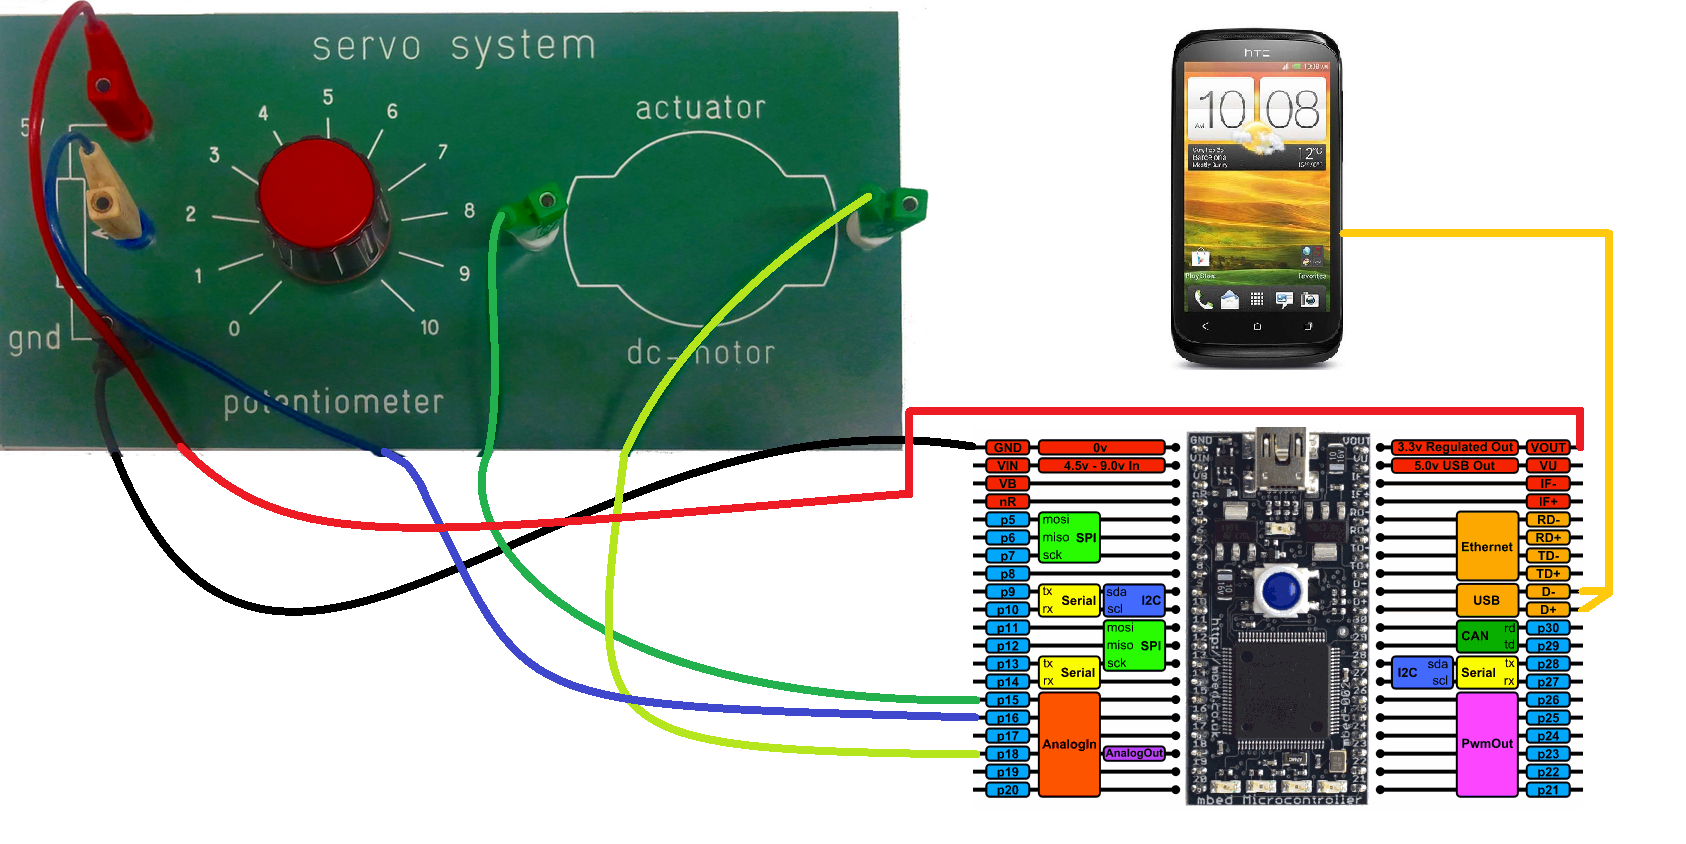
\includegraphics[width=0.8\textwidth]{imgs/opstelling.png}
		\caption{Opstelling}
		\label{fig:opstelling}
	\end{figure}
		\newpage
	\section{Onderzoek}
		\subsection{Servo systeem}
		Het is noodzakelijk eerst te onderzoeken hoe het servo systeem werkt. De analoog zichtbare waardes op het servo systeem lopen van 0 tot 10. De potentiometer geeft echter een waarde tussen 0 en 1 af aan de mbed. om het verband tussen de analoge waarde en de mbed te bepalen moeten er metingen worden gedaan. De knop op het servo systeem kan op een bepaalde stand worden geplaatst. Vervolgens kan de waarde van de potentiometer getoond worden. Er worden elf metingen gedaan vanaf de waarde 0 tot en met 10. De waarden zijn terug te vinden in tabel \ref{tab:gemeten}, de bijbehorende grafiek staat in figuur \ref{fig:logaritmisch}. Uit de gemeten waarden valt af te lezen dat het servo systeem exponentieel in waarde stijgt in plaats van lineair. Aan de hand van een vergelijking zou de waarde geschat kunnen gaan worden die de servo moet gaan aannemen bij de bijbehorende analoge stand. Het blijkt echter beter te werken om lineair te interpoleren tussen bekende waardes. De code hiervoor is te zien als snippet in listing \ref{lst:interpolate}\\
	\begin{table}[h]
		\begin{centering}
			\begin{tabular}{| c | c |}
				\hline
				Analoge waarde & Potentiometer waarde \\ \hline\hline
				1 & 0.002 \\\hline
				2 & 0.0062 \\\hline
				3 & 0.018 \\\hline
				4 & 0.059 \\\hline
				5 & 0.105 \\\hline
				6 & 0.2 \\\hline
				7 & 0.302 \\\hline
				8 & 0.504 \\\hline
				9 & 0.745 \\\hline
				10 & 0.996 \\
				\hline
			\end{tabular}
			\caption{Gemeten waarden}
			\label{tab:gemeten}
		\end{centering}
	\end{table}
	\begin{figure}[h]
		\centering
		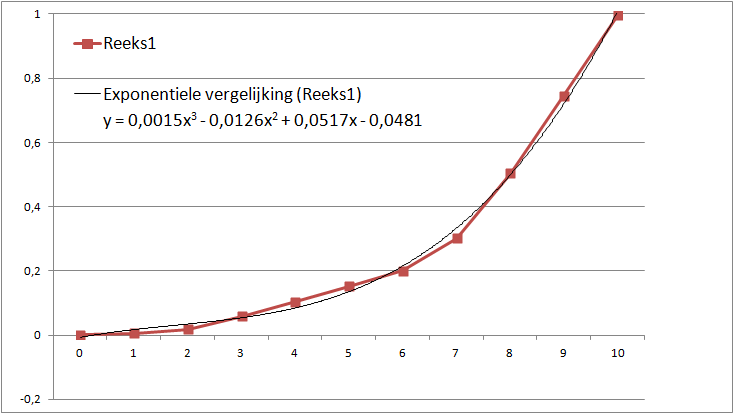
\includegraphics[scale=0.8]{imgs/logaritmisch.png}
		\caption{Exponentiele vergelijking}
		\label{fig:logaritmisch}
	\end{figure}
	\newpage
	\begin{lstlisting}[caption=Linear Interpolation, label=lst:interpolate, numbers=left]
	float interpolate(float x) {
		const float values[] = { 0.002, 0.0062, 0.018, 0.059, 0.105, 0.152,
					    0.2, 0.302, 0.504, 0.745, 0.996};
		if(x < 0 || x > 10.0) {
			return -1.0;
		}
		float ind = floor(x);
		int indi = (int) ind;
		if(ind == x) {
			return values[indi];
		}
		float low = values[indi];
		float high = values[indi + 1];
		float shift = x - ind;
		return (high - low) * shift + low;
	}
	\end{lstlisting}
		\subsection{Android}
		Nu bekend is hoe de analoge waarden omgezet worden naar digitale waarden kan een Android applicatie bedacht worden waarmee deze waarde aangepast kan gaan worden. Om te beginnen is hier een layout voor nodig met enkele eenvoudige mogelijkheden. De twee voor de hand liggende manieren om de servo mee te bedienen is een slider en twee knoppen om mee naar links of naar rechts te bewegen. De slider kan gebruikt worden om snel naar elke waarde te veranderen. De twee knoppen verhogen of verlagen de analoge waarde steeds met 0.1. De slider moet ook meeveranderen als deze knoppen gebruikt worden. De waarde die het servo systeem vervolgens moet aannemen moet ook zichtbaar gemaakt worden aan de gebruiker. Op figuur \ref{fig:layout1} is te zien hoe deze layout er uit ziet.
	\begin{figure}[h]
		\centering
		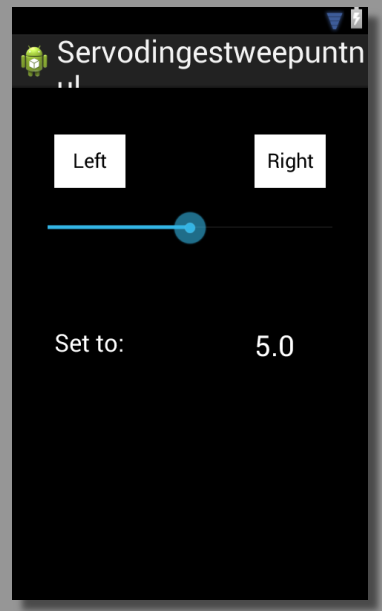
\includegraphics[scale=0.6]{imgs/layout1.png}
		\caption{Basis Layout}
		\label{fig:layout1}
	\end{figure}
		\subsection{Communicatie naar de mbed}
			De door de gebruiker gesette waarde is een integer tussen 0 en 100. Deze waarde wordt omgezet in een byte en kan dvervolgens naar de mbed gestuurd worden. In de mbed wordt vervolgens de waarde door 10 gedeeld om de gewenste analoge stand te verkrijgen. Met deze gewenste analoge waarde moet vervolgens de juist waarde voor de potentiometer gevonden worden tussen 0 en 1. Er zijn echter maar elf digitale waarden bekend die bij anaolge waarden horen. Door middel van lineaire interpolatie kan de juiste waarde voor de potentiometer gevonden worden zoals te zien in code snippet \ref{lst:interpolate}. Deze gevonden waarde wordt vervolgens gezocht door de mbed code. 
De potentiometer is echter niet accuraat genoeg om deze waarde altijd exact te vinden. Dit resulteert in het continu blijven veranderen van de stand van de as van het servo systeem. Om dit tegen te gaan wordt gebruik gemaakt van een margin rondom deze waarde. Een margin van 5\% boven en onder de waarde is voldoende om analoog niet het verschil te kunnen zien. Echter is een verschil van 5\% minder accuraat als de analoge waarde kleiner is. Dit komt door de exponentiele manier waarop het servo systeem zich gedraagt.

		\subsection{Communicatie naar de Android}
			De gebruiker wil echter ook weten wat momenteel de analoge stand is. Hiervoor moet de layout uitgebreid worden met een extra tekstveld. De nieuwe layout is te zien in figuur \ref{fig:layout2}. De potentiometer geeft een waarde tussen 0 en 1. Om hieruit de analoge waarde terug te krijgen moet inverse lineaire interpolatie worden toegepast, zoals te zien in listing \ref{lst:revinterpolate}. Op deze manier wordt een waarde gevonden tussen 0 en 10. Om de gebruiker in \'e\'en decimaal nauwkeurig te vertellen wat de huidige analoge waarde is wordt de gevonden waarde tussen 0 en 10 met 10 vermenigvuldigd. Deze waarde wordt dan omgezet naar een byte, waarna deze terug gestuurd kan worden naar de Android. Op de android wordt de waarde omgezet naar een float en weer door 10 gedeeld. Om het systeem niet te overbelasten wordt niet continu teruggestuurd wat de huidige anaolge waarde is maar wordt een interval van 0.5 seconde gebruikt.
	\begin{lstlisting}[caption=Linear Interpolation, label=lst:revinterpolate, numbers=left]
	float rev_interpolate(float x) {
		const float values[] = { 0.002, 0.0062, 0.018, 0.059, 0.105, 0.152,
					    0.2, 0.302, 0.504, 0.745, 0.996};
		int ind = 0;
		for(int i = 0; i < 10; i++){
			if(x >= values[i] && x <= values[i+1]){
				ind = i;
			}
		}
		if(x > values[10])
			return 10;
		if(x == values[ind])
			return ind;
		if(x == values[ind+1])
			return ind+1;
		float difference = fabs(values[ind+1] - values[ind]);
		return ind + (x-values[ind])/difference;
	}
	\end{lstlisting}
	\begin{figure}[h]
		\centering
		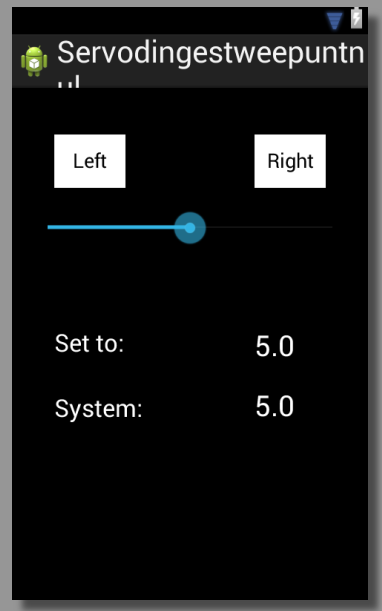
\includegraphics[scale=0.6]{imgs/layout2.png}
		\caption{Layout met huidige analoge waarde}
		\label{fig:layout2}
	\end{figure}
		\newpage
		\subsection{Besturing vanaf tweede toestel}
			Als laatste moet contact tussen Androids mogelijk worden. Een voor de hand liggende oplossing is een client server model. Waarbij de Android die aangesloten is op de mbed functioneert als server en andere Android apparaten als client. Dit leek het makkelijkste te gaan via het draadloos netwerk. Eerst moet er bekeken worden of het Android apparaat een client of een server wordt. Als de Android is aangesloten op een ander apparaat door middel van een USB kabel, is het een server. Anders is het apparaat een client. Voorlopig was de server gehardcode op een vast ip adres. De eerste berichten konden al uitgewisseld worden tussen de apparaten. De gesette waarde veranderd snel en goed mee. Echter werd toen aangegeven dat het niet toegestaan was om via het draadloze netwerk onderlinge communicatie te regelen. Het moest gedaan worden via Bluetooth.\\
Een deel moest hierdoor aangepast worden. Bluetooth gebruikt andere permissies en legt op een andere manier contact. Het gehardcode ip adres wordt vervangen voor een Bluetooth device naam met daarin een aangegeven waarde. Door de verbinding met bluetooth hebben de Android apparaten langer nodig om de juiste verbinding met elkaar te leggen. Er moet eerst gescand worden en toestemming worden verleend voordat er communicatie mogelijk is. Het omschrijven naar connectie met Bluetooth neemt veel tijd in beslag, waardoor het alleen mogelijk is om de gesette waarde heen en weer te communiceren. Deze communicatie is daarnaast niet extreem snel, waardoor er vertraging ontstaat in het verzenden van client naar server en omgekeerd. De slidebar die een nieuwe waarde wil aannemen op het tweede toestel ontvangt niet direct een nieuwe waarde waardoor de oude waarde terug wordt gecommuniceerd en de slidebar in een staat van onwetendheid komt. De slidebar schiet dan heen en weer omdat signalen elkaar tegenspreken. Het uitwisselen van gegevens is alleen getest voor koppeling tussen twee telefoons. De uiteindelijke layout is te zien in figuur \ref{fig:layout3}
	\begin{figure}
		\centering
		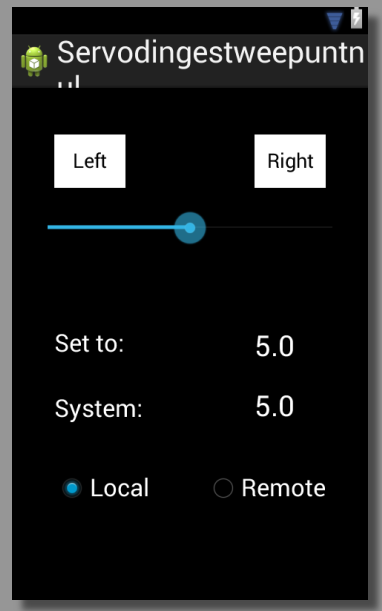
\includegraphics[scale=0.6]{imgs/layout3.png}
		\caption{Layout voor Server en Client}
		\label{fig:layout3}
	\end{figure}
	\newpage
	\section{Resultaat}
		\subsection{Werkende onderdelen}
			Uiteindelijk is het mogelijk geworden om via de potentiometer de waarde van het servo systeem door te geven aan de mbed. De mbed kan aan de hand van de waarde op de potentiometer de as van het servo systeem verplaatsen in de juiste richting, om de gewenste waarde te bereiken. Deze gesette waarde wordt naar de mbed gecommuniceerd aan de hand van een Android telefoon, waar de waarde wordt geregeld door middel van twee afstel knoppen of een slidebar. De mbed communiceert naar de Android wat de huidige zichtbare analoge waarde is, dit wordt bepaald aan de invers geinterpoleerde waarde van de huidige potentiometer waarde. En tot slot is het mogelijk om de Android die aan de mbed vast zit te besturen aan de hand van een tweede Android apparaat. Op dit tweede apparaat valt alleen de gesette waarde af te lezen. Het blijft wel mogelijk de waarde te setten op de Android die wel aan de mbed vast ligt. De uiteindelijkegrafische layout is te zien in figuur \ref{fig:layout3}
		\subsection{Verbeteringen}
			Momenteel zitten er in het systeem nog kleine onzuiverheden, daarnaast kan het geheel nog uitgebreid worden. Hieronder bevindt zich een lijst met mogelijke aanpassingen en verbeteringen. Deze bevinden zich in een volgorde van belangrijk naar minder belangrijk.
			\begin{itemize}
				\item Protocol maken voor onderlinge Bluetooth communicatie om meer gegevens uit te kunnen wisselen tussen server en client
				\item Ervoor zorgen dat de server elk willekeurig apparaat kan zijn, zonder een specifieke string in zijn device naam.
				\item Extra mogelijkheden maken voor de applicatie, zoals foutmeldingen binnen het systeem tonen aan de gebruiker, of aangeven dat er nog gescand wordt naar andere Bluetooth systemen.
				\item Code opschonen
				\item Mooier maken van de layout. Bijvoorbeeld door middel van een achtergrond en een startscherm.
			\end{itemize}
	\section{Logboek}
		\subsection{Maandag 3 Juni}
			Begonnen met het vertrouwt raken met de mbed. Enkele oefenprogramma's gemaakt die aangestuurd konden worden door middel van knopjes op de mbed zelf. Een aparte verandering in voltage naar analoge waarde waar genomen. Echter nog geen mogelijkheid gehad om waardes van de mbed naar de computer te krijgen. De lab machines die gebruikt konden worden hadden hiervoor geen permissies en er was geen eigen laptop meegenomen. Als tijdige oplossing output gecreerd door signalen met de LED lampjes.
		\subsection{Dinsdag 4 Juni}
			Programma's aan de praat gekregen die communiceren met een laptop. Juiste voltage en analoge waarde grafiek opgesteld. Android omgeving geinstalleerd. De voorbeeldcode voor een Android applicatie gecombineerd met mbed code onderzocht. Vervolgens begonnen met de layout van de Android applicatie en de mogelijkheden die er in de Android applicatie moeten komen.
		\subsection{Woensdag 5 Juni}
			Applicatie voor de Android werkend gekregen. De applicatie kan nu waardes aan de mbed doorgeven. De mbed zoekt vervolgens met deze waarde de juiste positie voor de as van de elektromotor. Begonnen met een server client systeem voor wifi. De android die aangesloten staat op de mbed functioneert als server. Andere android toestellen met dezelfde applicatie zouden contact moeten kunnen leggen met deze android om de waardes van servo aan te kunen passen. Dit werkt echter nog niet.
		\subsection{Donderdag 6 Juni}
			Bijwerken en opschonen van het LabReport. Debugging lines toegevoegd aan de client server code voor de applicatie.
		\subsection{Vrijdag 7 Juni}
			Het client server systeem werkend gekregen voor wifi. Vervolgens deze code verwijderd, wifi mocht niet gebruikt worden. Er toen voor gezorgd dat de mbed de huidige analoge waarde terug kan communiceren met het Android apparaat. Tot slot het client server model teruggehaald en omgeschreven voor communicatie voor bluetooth. Wegens tijdgebrek geen protocol gemaakt, waardoor het alleen mogelijk is de gesette waarde over en weer te sturen.
		\subsection{Zaterdag 8 Juni}
			Commentaar bij de code toegevoegd en het LabReport afgemaakt.
	
\end{document}